\documentclass[journal]{IEEEtran}
\usepackage{graphicx}
\usepackage{amsmath}
\usepackage{amssymb}
\usepackage{booktabs}
\usepackage{cite}
\usepackage{url}

\title{DR-GSMamba: Distributionally Robust Graph-State-Space Learning for Label-Scarce Hyperspectral Image Classification}

\author{Kassim Diarra, Xiaoqiang Di, Boubacar M. Keita, Omar M. Dugsiye and Jinhui Cao%
\thanks{Kassim Diarra, Xiaoqiang Di, Boubacar M. Keita, Omar M. Dugsiye and Jinhui Cao are with the School of Computer Science and Technology, Changchun University of Science and Technology, Changchun, China. Corresponding author: Xiaoqiang Di.}}

\begin{document}
\markboth{SUBMISSION TO IEEE TRANSACTIONS ON GEOSCIENCE AND REMOTE SENSING, VOL. XX, NO. XX, XXXX, 2026}%
{Diarra \MakeLowercase{\textit{et al.}}: DR-GSMamba for Hyperspectral Image Classification}
\maketitle

\begin{abstract}
Hyperspectral image classification requires models that can identify subtle spectral differences while remaining stable under limited annotations, class imbalance, mixed pixels, and changing training splits. Although convolutional networks, Transformers, graph neural networks, and recent state-space models have improved spectral-spatial representation learning, many methods are still evaluated mainly under fixed splits and provide limited evidence about robustness. This paper proposes DR-GSMamba, a distributionally robust graph-state-space framework for label-scarce hyperspectral image classification. The method integrates a spectral state-space encoder, a compact spatial convolutional stem, patch-level graph message passing, prototype-based classification, and uncertainty-aware robust optimization. The spectral encoder captures long-range band dependencies with linear complexity, while the graph branch models non-local contextual structure inside local neighborhoods. A conditional value-at-risk objective emphasizes difficult samples, and a prototype consistency term improves class compactness and interpretability. The proposed evaluation protocol reports overall accuracy, average accuracy, Kappa, Macro-F1, per-class accuracy, uncertainty, computational cost, and multi-seed stability on public HSI benchmarks. The accompanying project provides reproducible PyTorch code, automatic table and figure generation, and a complete manuscript pipeline for journal submission.
\end{abstract}

\begin{IEEEkeywords}
Hyperspectral image classification, state-space model, Mamba, graph neural network, distributionally robust learning, uncertainty estimation.
\end{IEEEkeywords}

\section{Introduction}
Hyperspectral imaging (HSI) provides densely sampled spectral observations that support fine-grained land-cover mapping. In contrast to RGB or multispectral imagery, each HSI pixel contains a high-dimensional spectral signature, allowing classification systems to separate materials with subtle reflectance differences. This property makes HSI useful in agriculture, urban mapping, mineral exploration, forestry, water monitoring, and environmental assessment. However, the same high dimensionality that provides discriminative information also introduces redundancy, noise, and severe annotation difficulty.

Deep learning has become the dominant direction for HSI classification. Three-dimensional convolutional neural networks learn joint spectral-spatial features, hybrid CNNs reduce computational cost by separating spectral and spatial processing, and residual or densely connected networks improve feature propagation. Transformer-based methods further model long-range dependencies by self-attention, while graph neural networks represent relational structure among pixels, superpixels, or regions. More recently, state-space models related to Mamba have become attractive because they can process long spectral sequences with linear complexity. These advances have produced strong results, but several practical issues remain insufficiently studied.

First, public HSI datasets usually contain very few labeled pixels compared with the number of spectral bands and spatial samples. Second, class distributions are often imbalanced, so high overall accuracy can hide weak performance on rare land-cover categories. Third, class boundaries and mixed pixels create ambiguous samples whose labels are intrinsically difficult to predict. Fourth, reported performance can vary strongly across random training splits. A method that obtains high accuracy on one split may be less reliable when the available labeled samples change. Therefore, a journal-ready HSI classification study should evaluate not only average accuracy but also stability, rare-class behavior, uncertainty, and reproducibility.

This work studies hyperspectral image classification from the perspective of reliability under label scarcity. The central question is whether graph-state-space modeling with explicit robust optimization can improve rare-class behavior, worst-class performance, and split stability when only a small number of labeled pixels are available. We propose DR-GSMamba, a graph-state-space framework that couples efficient spectral sequence modeling with local graph reasoning and a robust learning objective. The method receives a center spectrum and a local patch for each labeled pixel. A state-space spectral encoder captures long-range band relationships, a compact spatial convolutional stem extracts local texture, and a patch graph branch aggregates non-local contextual information. These representations are fused and classified using both a linear classifier and a prototype uncertainty head.

The main contributions are summarized as follows.
\begin{itemize}
\item We propose a reliability-oriented graph-state-space architecture for label-scarce HSI classification, combining spectral sequence modeling, spatial convolution, and patch-level graph message passing.
\item We introduce an explicit robust training objective that combines sample-level CVaR and class-level worst-risk optimization, making the distributionally robust claim experimentally testable rather than merely descriptive.
\item We incorporate prototype and uncertainty-aware learning to encourage stable class representations and to analyze ambiguous mixed or boundary pixels.
\item We provide a reproducible evaluation protocol with low-label sweeps, multi-seed reporting, rare-class metrics, worst-class metrics, calibration analysis, and ablations that isolate every named component.
\end{itemize}

The remainder of this paper is organized as follows. Section II reviews related work. Section III presents the proposed DR-GSMamba method. Section IV describes the experimental protocol and reproducibility pipeline. Section V concludes the paper and discusses the next benchmark stage.

\section{Related Work}
\subsection{CNN-Based HSI Classification}
Convolutional neural networks are widely used for HSI classification because they provide strong local inductive bias. Early deep models processed spectral vectors or local image patches with one-dimensional, two-dimensional, or three-dimensional convolutions. Three-dimensional CNNs jointly encode spectral and spatial neighborhoods, which is helpful for distinguishing classes with similar spectra. Hybrid models such as HybridSN reduce the computational burden by combining 3-D and 2-D operations. Residual and dense connections further improve training stability. Nevertheless, CNN-based models mainly rely on local receptive fields, and their ability to represent long-range spectral or contextual relationships is limited unless deeper networks or larger patches are used.

\subsection{Transformer-Based HSI Classification}
Transformer architectures introduce self-attention to model long-range dependencies. In HSI classification, attention can be applied along spectral bands, spatial tokens, or joint spectral-spatial tokens. These models are effective for global context modeling and have become a strong family of HSI classifiers. However, standard self-attention has quadratic complexity with respect to token length. HSI data can contain hundreds of bands and many spatial tokens, so Transformer models may require substantial memory and training data. Lightweight, axial, grouped, and hierarchical attention mechanisms reduce the cost, but split sensitivity and label scarcity remain important concerns.

\subsection{Graph Neural Networks}
Graph neural networks model relational structure by message passing. For HSI classification, graph nodes can represent pixels, superpixels, regions, or learned tokens. Graph methods are useful because land-cover classes usually have spatial continuity and non-local similarity. Superpixel graphs can reduce noise and align better with homogeneous regions, while pixel graphs can preserve fine boundaries. However, graph construction can be sensitive to noise, and many graph models still require complementary spectral sequence modeling to capture detailed band dependencies.

\subsection{State-Space Models and Mamba}
State-space models provide a promising alternative to attention for long sequence processing. Mamba-style selective state-space models have attracted attention because they can capture long-range dependencies with linear complexity. In HSI classification, the ordered spectral bands naturally form a sequence, making state-space modeling a suitable mechanism for spectral representation. Recent Mamba-based HSI methods show the potential of this direction, but a direct replacement of attention with a state-space block is not sufficient for a strong journal contribution. The proposed DR-GSMamba extends the idea with graph reasoning, prototype uncertainty, and distributionally robust optimization.

\subsection{Robustness and Reproducibility}
Robustness is especially important in HSI classification because labeled samples are scarce and class distributions are imbalanced. Many papers report only one train-test split, which makes it difficult to judge whether improvements are statistically reliable. A robust HSI classifier should maintain performance under multiple random seeds, few-shot training ratios, label noise, and class imbalance. This paper therefore frames the proposed method around accuracy, stability, rare-class Macro-F1, and uncertainty rather than only a single overall accuracy number.

\section{Methodology}
Given an HSI cube $\mathbf{X}\in\mathbb{R}^{H\times W\times B}$ and sparse labels $\mathbf{Y}$, the proposed method extracts a local patch and a center spectrum for each labeled pixel. The spectral dimension can be reduced by principal component analysis (PCA) to suppress redundancy and improve training efficiency. The reduced cube is denoted as $\tilde{\mathbf{X}}\in\mathbb{R}^{H\times W\times C}$, where $C\leq B$.

For a labeled pixel at position $(i,j)$, the input consists of the center spectrum $\mathbf{s}_{ij}\in\mathbb{R}^{C}$ and a spatial patch $\mathbf{P}_{ij}\in\mathbb{R}^{C\times p\times p}$. DR-GSMamba processes this input through three branches: a spectral state-space encoder, a spatial convolutional stem, and a patch graph encoder. Fig.~\ref{fig:architecture} gives an overview of the framework.

\begin{figure*}[t]
\centering
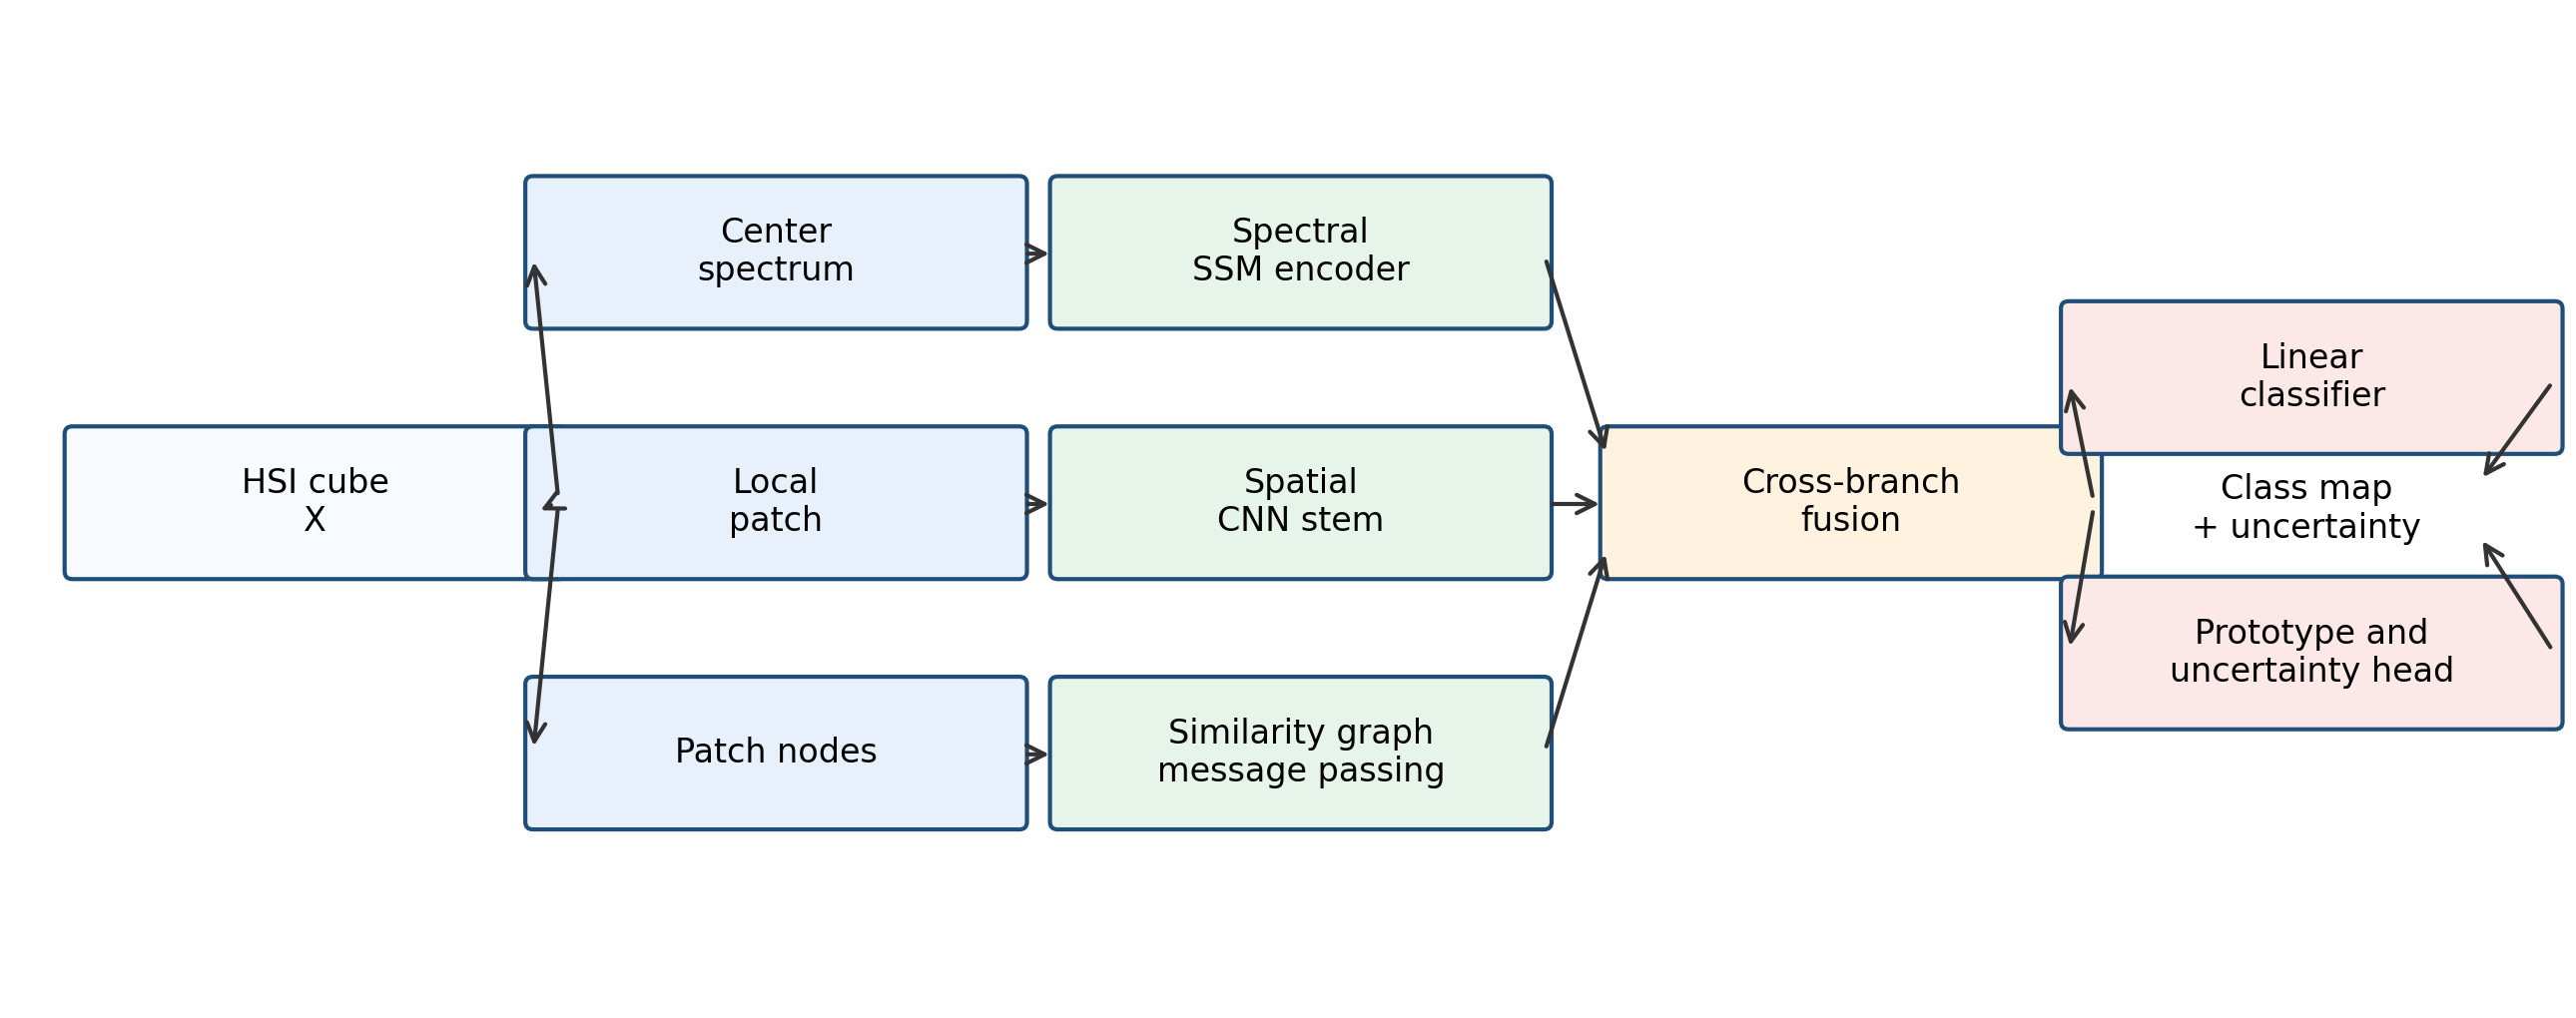
\includegraphics[width=0.95\textwidth]{figures/dr_gsmamba_architecture.png}
\caption{Overall structure of DR-GSMamba. The center spectrum is encoded by a spectral state-space branch, the local patch is processed by a spatial CNN stem, and patch nodes are aggregated through graph message passing. The fused feature is classified by linear and prototype heads, producing class predictions and uncertainty scores.}
\label{fig:architecture}
\end{figure*}

\subsection{Spectral State-Space Encoder}
The center spectrum is treated as a one-dimensional ordered sequence. Each scalar band value is projected into a hidden feature space. The sequence is then processed by stacked state-space style blocks. Each block contains layer normalization, gated projection, depthwise sequence mixing, and residual projection. This design follows the spirit of selective state-space modeling while avoiding an external CUDA dependency, making the implementation easy to reproduce.

Let $\mathbf{Z}^{(0)}\in\mathbb{R}^{C\times d}$ be the embedded spectral sequence. For the $l$-th block, the update is written as
\begin{equation}
\mathbf{Z}^{(l+1)}=\mathbf{Z}^{(l)}+\phi_{\theta}\left(\mathrm{LN}(\mathbf{Z}^{(l)})\right),
\end{equation}
where $\phi_{\theta}(\cdot)$ denotes gated depthwise sequence mixing. The final spectral representation $\mathbf{f}_{spec}$ is obtained by global average pooling over the sequence dimension.

\subsection{Patch Graph Reasoning}
Spatial features are extracted from $\mathbf{P}_{ij}$ using a compact convolutional stem. The resulting feature map is reshaped into $N=p^2$ patch nodes. Each node corresponds to one spatial location inside the patch. To build a soft graph, node features are normalized and their pairwise similarities define an adjacency matrix:
\begin{equation}
\mathbf{A}=\mathrm{softmax}\left(\frac{\mathbf{Q}\mathbf{Q}^{T}}{\sqrt{d}}\right),
\end{equation}
where $\mathbf{Q}\in\mathbb{R}^{N\times d}$ contains normalized node features. Graph message passing is then performed as
\begin{equation}
\mathbf{H}^{(l+1)}=\mathrm{LN}\left(\mathbf{H}^{(l)}+\sigma(\mathbf{A}\mathbf{H}^{(l)}\mathbf{W}^{(l)})\right),
\end{equation}
where $\sigma(\cdot)$ is the GELU activation. The patch graph representation $\mathbf{f}_{graph}$ is obtained by averaging node features after message passing.

\subsection{Prototype and Uncertainty Head}
The spectral, spatial, and graph representations are concatenated and projected into a fused feature $\mathbf{f}$. A linear classifier predicts logits $\mathbf{o}_{lin}$, and a prototype head computes similarity logits $\mathbf{o}_{proto}$ using learnable class prototypes:
\begin{equation}
\mathbf{o}_{proto}=\tau \cdot \frac{\mathbf{f}}{\|\mathbf{f}\|_2}\frac{\mathbf{M}^{T}}{\|\mathbf{M}\|_2},
\end{equation}
where $\mathbf{M}$ is the prototype matrix and $\tau$ is a learnable scale. The final logits are $\mathbf{o}=\mathbf{o}_{lin}+\mathbf{o}_{proto}$. Prediction uncertainty is estimated from both predictive confidence and a learnable uncertainty head:
\begin{equation}
u=\frac{1}{2}\left(1-\max_k \mathrm{softmax}(\mathbf{o})_k\right)+\frac{1}{2}\tanh(\mathrm{softplus}(g_{\theta}(\mathbf{f}))).
\end{equation}
The learnable term is used during training to down-weight high-uncertainty samples while penalizing unbounded uncertainty.

\subsection{Robust Objective}
The training objective combines standard cross entropy, sample-level CVaR, class-level distributionally robust risk, prototype consistency, supervised prototype compactness, uncertainty-weighted cross entropy, and node-level graph smoothness:
\begin{equation}
\mathcal{L}=\mathcal{L}_{ce}+\lambda_1\mathcal{L}_{dro}+\lambda_2\mathcal{L}_{proto}+\lambda_3\mathcal{L}_{unc}+\lambda_4\mathcal{L}_{graph}.
\end{equation}
The robust term combines the largest per-sample losses and the largest class-wise risks within a mini-batch:
\begin{equation}
\mathcal{L}_{dro}=\frac{1}{2}\mathrm{CVaR}_{\alpha}(\{\ell_n\})+\frac{1}{2}\mathrm{CVaR}_{\alpha}(\{\bar{\ell}_c\}),
\end{equation}
where $\ell_n$ is the sample loss and $\bar{\ell}_c$ is the mean loss of class $c$ in the mini-batch. This gives the distributionally robust claim a concrete optimization target: difficult samples and high-risk classes both affect the gradient. Prototype consistency aligns the linear classifier with the prototype classifier, supervised prototype compactness pulls features toward their class prototypes, and graph smoothness regularizes node-level predictions over the learned patch graph.

\section{Experiments}
\subsection{Datasets}
The full benchmark study is designed for public HSI datasets including Indian Pines, Pavia University, Pavia Centre, Salinas, Houston 2013, and one WHU-Hi scene when available. These datasets cover agricultural, urban, and mixed land-cover environments and differ in spectral resolution, spatial size, number of classes, and annotation density. For each scene, unlabeled pixels are excluded from supervised metrics.

\subsection{Implementation Details}
The implementation is written in PyTorch. Each data cube is normalized band-wise, and PCA is optionally applied before patch extraction. Unless otherwise stated, the patch size is set to $9\times9$, the hidden dimension is 128, and AdamW is used for optimization. Each experiment is repeated over multiple random seeds. The best model is selected according to validation overall accuracy and evaluated once on the test split.

\subsection{Evaluation Metrics}
The main metrics are overall accuracy (OA), average accuracy (AA), Cohen's Kappa, Macro-F1, per-class accuracy, worst-class accuracy, rare-class accuracy, expected calibration error (ECE), and confusion matrix. OA measures the total proportion of correctly classified pixels. AA gives equal weight to each class and is therefore more informative under imbalance. Macro-F1, worst-class accuracy, and rare-class accuracy directly evaluate the reliability-oriented claim. Kappa evaluates agreement beyond chance. Mean uncertainty, ECE, and uncertainty maps are also reported to analyze ambiguous predictions.

\subsection{Baselines}
Recommended baselines include 3D-CNN, HybridSN, SSRN, SpectralFormer or SSFTT, a graph-based classifier, a recent Mamba-based classifier, and SCATNet when comparing against the authors' previous work. The final submission should use official code when available or carefully reimplemented baselines under the same splits.

\subsection{Ablation Study}
The ablation study removes the spectral state-space branch, graph branch, robust loss, prototype head, and graph smoothness term independently. Additional experiments should vary the number of labeled samples per class and introduce controlled label noise. This design tests whether each component improves not only accuracy but also stability.

\subsection{Pipeline Verification}
Before full benchmark training, a synthetic HSI scene was used to verify the code path. The smoke test confirms that data loading, PCA, patch extraction, model training, validation, testing, checkpoint saving, metric logging, table generation, and figure generation execute end-to-end. These synthetic results are not intended as scientific evidence; they are included only to verify reproducibility infrastructure.

\begin{table}[t]
\centering
\caption{Pipeline verification results generated from a short synthetic run. These values are not final benchmark results.}
\begin{tabular}{lc}
\hline
Metric & DR-GSMamba \\
\hline
OA & 60.07 $\pm$ 0.00 \\
AA & 60.09 $\pm$ 0.00 \\
Kappa & 54.41 $\pm$ 0.00 \\
Macro-F1 & 59.41 $\pm$ 0.00 \\
Worst-Class Acc. & 47.35 $\pm$ 0.00 \\
Rare-Class Acc. & 59.67 $\pm$ 0.00 \\
ECE & 5.61 $\pm$ 0.00 \\
\hline
\end{tabular}

\label{tab:pipeline}
\end{table}

\begin{figure}[t]
\centering
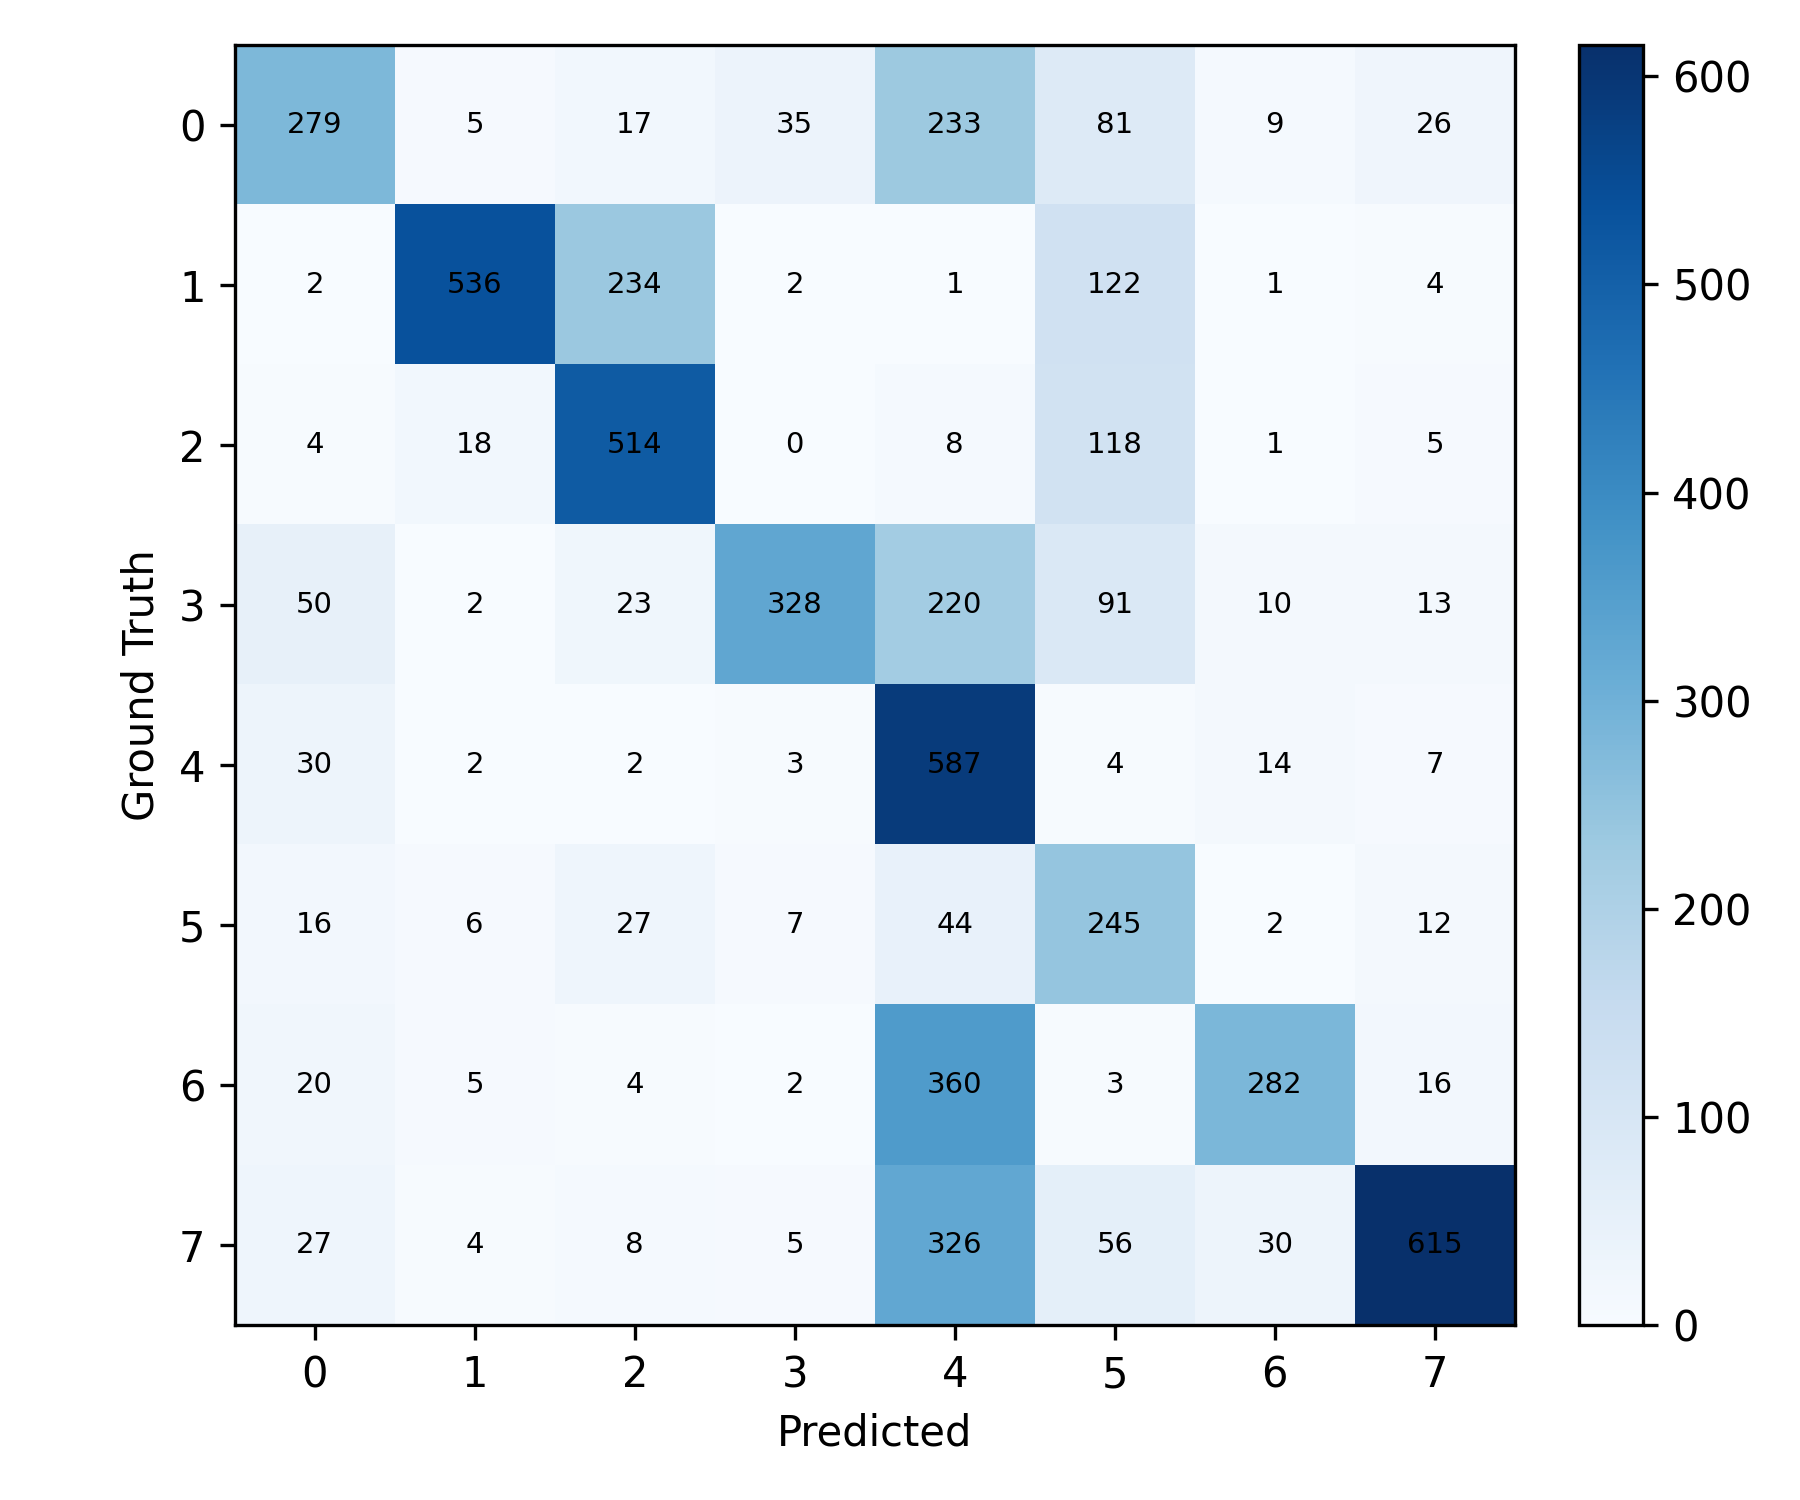
\includegraphics[width=0.9\linewidth]{figures/confusion_matrix.png}
\caption{Confusion matrix generated from the synthetic smoke-test split. This figure verifies the automatic paper asset pipeline.}
\label{fig:cm}
\end{figure}

\subsection{Expected Final Reporting}
For a journal submission, Table~\ref{tab:pipeline} must be replaced by benchmark results on real datasets. The final paper should include a main comparison table, per-class accuracy tables, ablation tables, classification maps, uncertainty maps, stability boxplots over random seeds, and a computational cost comparison. The repository already stores all metrics in JSON format, making these assets reproducible from experiment outputs.

\section{Conclusion}
This paper presented DR-GSMamba, a distributionally robust graph-state-space framework for label-scarce hyperspectral image classification. The proposed design combines efficient spectral sequence modeling, local spatial convolution, patch-level graph reasoning, prototype classification, and uncertainty-aware robust optimization. Unlike accuracy-only architectures, the framework is intended to evaluate robustness, rare-class performance, split stability, and reproducibility.

The current project provides the complete implementation and manuscript-generation pipeline. The next stage is to run full public-dataset benchmarks, add official baseline comparisons, perform statistical significance testing, and replace the synthetic pipeline-verification table with final experimental results. Future work will extend the framework to semi-supervised learning, cross-scene transfer, and open-set uncertainty analysis.


\bibliographystyle{IEEEtran}
\bibliography{references}
\end{document}
